%%%%%%%%%%%%%%%%%%%%%%%%%%%%%%%%%%%%%%%%%%%%%%%%%%%%%%%%%%%%%%%%
%%%%%%%%%%%%%%%%%%%%%%%%%%%%%%%%%%%%%%%%%%%%%%%%%%%%%%%%%%%%%%%%
%%%%
%%%% This text file is part of the source of slides for
%%%% `Introduction to High-Performance Scientific Computing'
%%%% by Victor Eijkhout, copyright 2012-2022
%%%%
%%%%%%%%%%%%%%%%%%%%%%%%%%%%%%%%%%%%%%%%%%%%%%%%%%%%%%%%%%%%%%%%
%%%%%%%%%%%%%%%%%%%%%%%%%%%%%%%%%%%%%%%%%%%%%%%%%%%%%%%%%%%%%%%%

\begin{numberedframe}{Classes of programming errors}
  Logic errors:\\
  functions behave differently from how you thought,\\
  or interact in ways you didn't envision

  Hard to debug
\end{numberedframe}

\begin{numberedframe}{More classes of errors}
  Coding errors:\\
  send without receive\\
  forget to allocate buffer

  Debuggers can help
\end{numberedframe}

\Level 2 {Defensive programming}

\begin{numberedframe}{Defensive programming}
  \begin{itemize}
  \item Keep It Simple (`restrict expressivity')
  \item Example: use collective instead of spelling it out
  \item easier to write / harder to get wrong\\
    the library and runtime are likely to be better at optimizing than you
  \end{itemize}
\end{numberedframe}

\begin{numberedframe}{Memory management}
  Beware of memory leaks:\\
  keep allocation and free in same lexical scope

  C++ does this automatically with RAII
\end{numberedframe}

\begin{numberedframe}{Modular design}
  Design for debuggability, also easier to optimize

  Separation of concerns: try to keep code aspects separate

  Premature optimization is the root of all evil (Knuth)
\end{numberedframe}

\begin{numberedframe}{MPI performance design}
  Be aware of latencies: bundle messages\\
  (this may go again separation of concerns)

  Consider `eager limit'

  Process placement, reduction in number of processes
\end{numberedframe}

\Level 2 {Debugging}

\begin{numberedframe}{}
\begin{quotation}
  Debugging is like being the detective in a crime movie where you are
  also the murderer. (Filipe Fortes, 2013)
\end{quotation}
What do you do when your program misbehaves?
\begin{itemize}
\item Insert print statements, recompile, run again.
\item Run your program in a debugger
\item (also: attach a debugger, inspect a core dump)
\end{itemize}
\end{numberedframe}

\begin{numberedframe}{Simple example: listing}
\codelisting{tutorials/gdb/c/hello.c}
\end{numberedframe}

\begin{numberedframe}{Simple example: running}
  \small
\begin{verbatim}
%% cc -g -o hello hello.c
# regular invocation:
%% ./hello
hello world
# invocation from gdb:
%% gdb hello
GNU gdb 6.3.50-20050815 # ..... [version info]
Copyright 2004 Free Software Foundation, Inc. .... [copyright info] ....
(gdb) run
Starting program: /home/eijkhout/tutorials/gdb/hello 
Reading symbols for shared libraries +. done
hello world

Program exited normally.
(gdb) quit
%%
\end{verbatim}  
\end{numberedframe}

\begin{numberedframe}{Source listing}
\begin{verbatim}
%% cc -o hello hello.c
%% gdb hello
GNU gdb 6.3.50-20050815 # ..... version info
(gdb) list
\end{verbatim}
Important to use the \n{-g} compile option!
\end{numberedframe}

\begin{numberedframe}{Run with arguments}
\codelisting{tutorials/gdb/c/say.c}
\begin{verbatim}
%% gdb say
.... the usual messages ...
(gdb) run 2
Starting program: /home/eijkhout/tutorials/gdb/c/say 2
Reading symbols for shared libraries +. done
hello world
hello world
\end{verbatim}
\end{numberedframe}

\begin{numberedframe}{Memory problems 1}
\verbatimsnippet{gdb-square}
\begin{verbatim}
%% cc -g -o square square.c
 %% ./square
5000
Segmentation fault
\end{verbatim}
The debugger will stop at the problem.
\end{numberedframe}

\begin{numberedframe}{Stack trace}
\begin{tabular}{cc}
  \toprule
  \multicolumn{2}{c}{Displaying a stack trace} \\
  \midrule
  gdb & lldb\\
  \midrule
  \n{(gdb) where}&\n{(lldb) thread backtrace}\\
  \bottomrule
\end{tabular}

{\small
\begin{verbatim}
(gdb) backtrace
#0  0x00007fff824295ca in __svfscanf_l ()
#1  0x00007fff8244011b in fscanf ()
#2  0x0000000100000e89 in main (argc=1, argv=0x7fff5fbfc7c0) at square.c:7
\end{verbatim}
}
\end{numberedframe}

\begin{numberedframe}{Inspecting a stack frame}
  \begin{tabular}{ll}
    \toprule
    \multicolumn{2}{c}{Investigate a specific frame}\\
    \midrule
    gdb&clang\\
    \n{frame 2}&\n{frame select 2}\\
    \bottomrule
  \end{tabular}

  Then \n{print} variables and such.
\end{numberedframe}

\begin{numberedframe}{Out-of-bounds errors}
\verbatimsnippet{gdb-up}
\end{numberedframe}

\begin{numberedframe}{Out of bounds in debugger}
\begin{verbatim}
Program received signal EXC_BAD_ACCESS, Could not access memory.
Reason: KERN_INVALID_ADDRESS at address: 0x0000000100200000
0x0000000100000f43 in main (argc=1, argv=0x7fff5fbfe2c0) at up.c:15
15          s += array[i];
(gdb) print array
$1 = (double *) 0x100104d00
(gdb) print i
$2 = 128608
\end{verbatim}    
\end{numberedframe}

\begin{numberedframe}{Breakpoints}
\begin{tabular}{ll}
  \toprule
  \multicolumn{2}{c}{Set a breakpoint at a line}\\
  \midrule
  gdb&lldb\\
  \n{break foo.c:12}&\n{breakpoint set [ -f foo.c ] -l 12}\\
  \bottomrule
\end{tabular}  
\end{numberedframe}

\begin{numberedframe}{Stepping}
\begin{tabular}{lll}
  \toprule
  \multicolumn{3}{c}{Stepping through a program}\\
  \midrule
  gdb&lldb&meaning\\
  \n{run}&&start a run\\
  \n{cont}&&continue from breakpoint\\
  \n{next}&&next statement on same level\\
  \n{step}&&next statement, this level or next\\
  \bottomrule
\end{tabular}
\end{numberedframe}

\Level 2 {Memory debugging}

\begin{numberedframe}{Program with problems}
\codelisting{tutorials/gdb/c/square1.c}  
\end{numberedframe}

\begin{numberedframe}{Valgrind output}
\begin{verbatim}
%% valgrind square1
==53695== Memcheck, a memory error detector
==53695== [stuff]
10
==53695== Invalid write of size 4
==53695==    at 0x100000EB0: main (square1.c:10)
==53695==  Address 0x10027e148 is 0 bytes after a block of size 40 alloc'd
==53695==    at 0x1000101EF: malloc (vg_replace_malloc.c:236)
==53695==    by 0x100000E77: main (square1.c:8)
==53695== 
\end{verbatim}  
\end{numberedframe}


\Level 2 {Parallel Debugging}

\begin{numberedframe}{Debugging}
  I assume you know about gdb and valgrind\ldots
  \begin{itemize}
  \item Interactive use of gdb, starting up multiple xterms\\
    feasible on small scale
  \item Use gdb to inspect dump:\\
    can be useful, often a program crashes hard and leaves no dump
  \end{itemize}
  Note: compile options \texttt{-g -O0}
\end{numberedframe}

\begin{numberedframe}{Parallel debuggers}
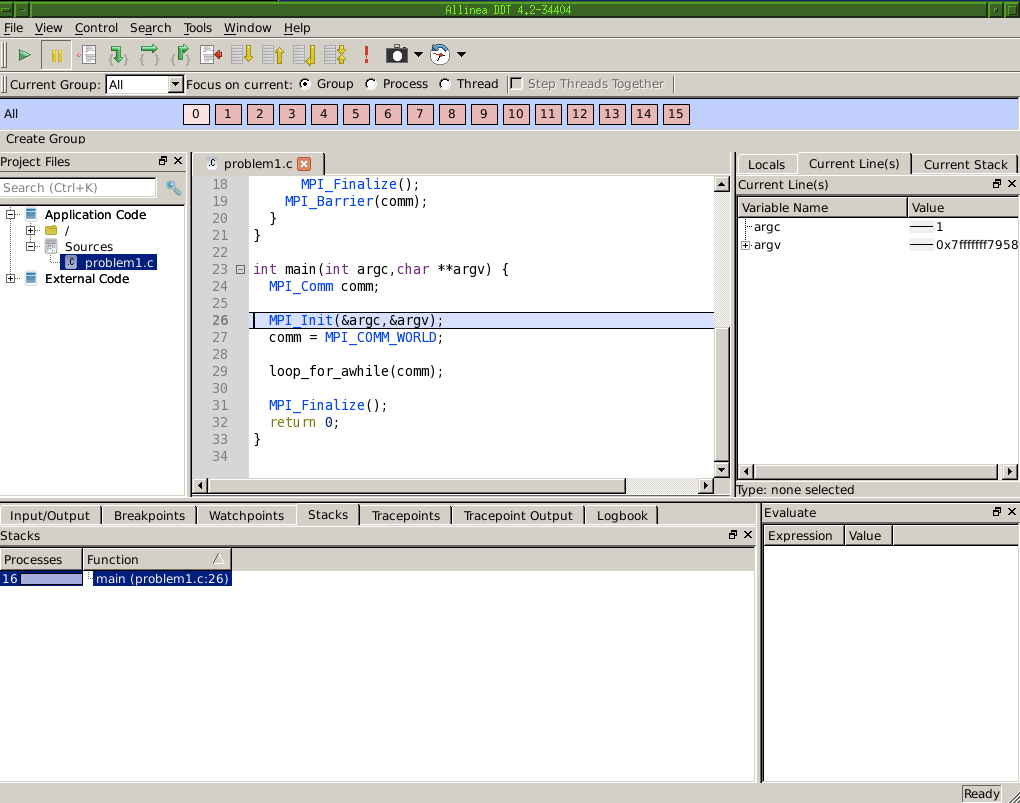
\includegraphics[scale=.3]{ddt1}
\end{numberedframe}

\begin{numberedframe}{Buggy code}
\begin{verbatim}
for (it=0; ; it++) {
  double randomnumber = ntids * ( rand() / (double)RAND_MAX );
  printf("[%d] iteration %d, random %e\n",mytid,it,randomnumber);
  if (randomnumber>mytid && randomnumber<mytid+1./(ntids+1))  
    MPI_Finalize();
  MPI_Barrier(comm);
}
\end{verbatim}
\end{numberedframe}

\begin{numberedframe}{Parallel inspection}
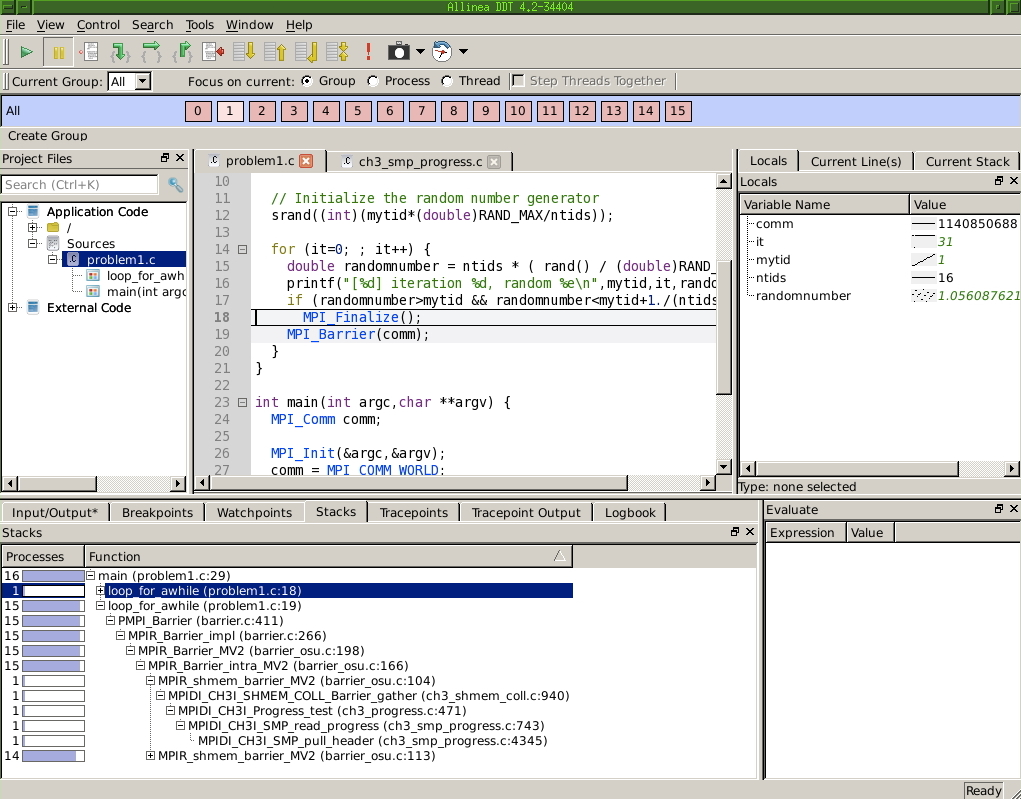
\includegraphics[scale=.3]{ddt2}
\end{numberedframe}

\begin{numberedframe}{Stack trace}
  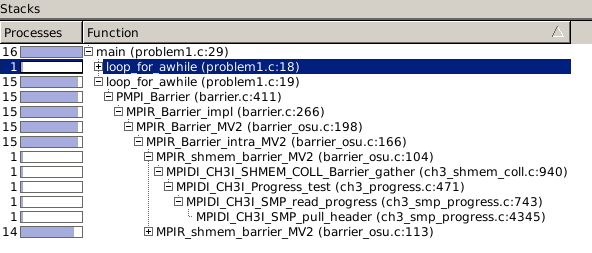
\includegraphics[scale=.5]{ddt3}
\end{numberedframe}

\begin{numberedframe}{Variable inspection}
  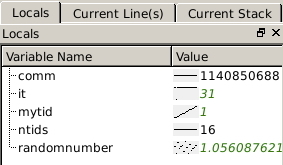
\includegraphics{ddt4}
\end{numberedframe}

